% This is the Latex template for my future homework write-ups
% A basic form of Latex command: '/command name[argu, argu]{argu*}' as below:
\documentclass[12pt, letterpaper]{article} % use 'tab' to complete 
% which means this document is an article with 12pt (font size) and letterpaper (paper type)


% ======================================================
% This is the preamble section for loading packages, a basic form looks like: 
% /usepackage{filename} the package name is the .sty file.  Let's load some 
% packages (Latex will complain if the .sty file is not in PWD):
% ======================================================
\usepackage{indentfirst} % indent the 1st line of the 1st paragraph, using \noindent to cancel
\usepackage{amsmath} % basic mathematic 
\usepackage{graphicx} % for using graphics
\usepackage{array} % for using arrays
\usepackage{lineno}   % for adding line numbers
\usepackage[authoryear]{natbib}   % for citing, more options see 'natbib'
\usepackage[notref,notcite]{showkeys} % easy to check the #name of each \ref
\usepackage{bm}  % Use the bold mode in math 
\usepackage{ulem} % added lines for our text, i.e., underline...
\usepackage{xcolor} % used for adding color to our text
\usepackage{listings} % used for displaying the highlight code

\usepackage{listings}
\usepackage{xcolor}

% ============================================================================
% These are basic settings for making title and content
% ============================================================================
% Now, we start the work by entering the document with:
\begin{document}  % always remember 'begin - end' pairs
% Basic settings for the title page
\title{\LaTeX: Phys 5391 Assignment - 5} % title name
\author{Yu Hong\\Space Physics Group} % double-slash for new line
\date{December 04, 2020}  % or the \today command to insert today's date.
% Now setting the format of the article
\maketitle % make a title based on  the info above
\newpage % make a new page
\tableofcontents % make a content page
\newpage % make a new page
\linenumbers % turn on the line numbers.




% ============================================================================
% This Section is used for demonstrating some basic command of controlling paragraph and texts
% ============================================================================

\section{Basic Information} % adding new section
\subsection{Programming Languages} % adding new subsections I
% add  a new paragraph
Currently I'm 50\% data \vspace{3mm} analyst \& 50\% model \hspace{5mm} simulator. % testing special symbols by adding '\'
% \vspace{3mm} and \hspace{5mm} are used to get space 
Specifically speaking, I use \textbf{python 2/3} for  \\ % or use \newline to start a new line 
\textit{data processing} and \emph{visualization}, I'm family with  % \textbf{}--> make bold;  \textit{} --> to emphasis
reading satellite data files like \textit{.cdf}, \textit{.netcdf} format and ground-based radar files like \textit{.hdf}. 
% \textit{} --> make italics;  \textsf{ } --> make Sans serif font
In the past I basically used \textbf{Matlab} and a little \textsf{IDL} regarding NASA SPEDAS packages, but now I 
% \textsc{} --> Capitalize all letters
am 100\% \textit{pythonic} dependent. In terms of numerical simulation, I use \textsc{Fortran 90} and work with \textbf{GITM}. 

A minimal model for the evolution of the global dynamical state of the magnetotail during the substorm, involving only three simple rules has been developed. The model considers the general state of the magnetospheric system rather than concentrate on the physical nature of the substorm instability. When driven by a real solar wind power input, the minimal substorm model produces a probability distribution of times between substorm onsets that compares favourably with the distribution of 1001 inter-substorm intervals found by Borovsky et al. from observation. In this paper we examine the validity of the assumptions behind the model, specifically that the integrated solar wind input between two contiguous substorm onsets is proportional to the solar wind input at the time of the first substorm. We do this by comparing the integrated solar wind input between pairs of substorm onsets with the solar wind input at the time of the first substorm onset for a set of observed substorm pairs.



% ============================================================================
% This Section used for writing mathematics stuffs, the equation and table will be showing here
% ============================================================================
\section{Math Environment} % Start a new section for math
My favorite physical equation comes from  \textit{Einstein's special relativity}. 

The equation: $E = mc\textsuperscript{2}$ indicates that the energy (E) and mass (m), 
which are definitely interchangeable. All mass objects in the world will have energy, 
the energy equals the mass times the speed of light ($\bm{c = 3\times10\textsuperscript{8} m/s}$) 
squared, which means energy and mass are different forms of the same thing. \\ % Inline math text is done easily with dollar signs

\begin{math}  % Note that \would also work instead of \begin and \end (math only)
  E = {mc}\textsuperscript{2} % \textsuperscript{} used to add superscript
\end{math} % end the environment {math}

In special relativity, the the relativistic mass, changes with its moving speed. 
Combine this variation with the equation $E = mc\textsuperscript{2}$, we can get: 

% use the environment {equation} and label the equation as equ1
\begin{equation} 
  E = \frac{mc^2}{\sqrt{1-\frac{v^2}{c^2}}}
  \label{eq:1}  
\end{equation} % end the environment {equation}

Here, m means the rest mass, c means the speed of light, which is 3x10\textsuperscript{8} m/s, and v is the speed 
of the object. I added a table to describe the corresponding variables in the equation above in 
Table \ref{tab:tab1}: % add a reference name ex1 to this table

% We'll see more of this syntax explained below (e.g., the !h).
\begin{table}[!h] % use the environment {table}
  \begin{center} % use the environment {environment}
  \begin{tabular}{|l|c|c|r|} % make a table with 4 colums: left, center, center, right
    \hline % Used to draw horizontal lines
    Var 1 & Var 2 & Var 3.1 & Var 3.2\\ % make a new line
    \hline % Used to draw horizontal lines
    \hline % Used to draw horizontal lines
    E & m &v & c\\ % make a new line
    \hline % Used to draw horizontal lines
    \hline % Used to draw horizontal lines
    energy & mass& speed of object & speed of light \\ % make a new line
    \hline % Used to draw horizontal lines
  \end{tabular} % end the environment {tabular}
  % Caption and label commands are key.
  \caption{The corresponding variables of the equation } % add caption to this table
  \label{tab:tab1} % label the table, when quoting, \label and \ref appear in pairs
  \end{center} % end the environment {center}
\end{table} % end the environment {table}





% ============================================================================
% This Section is used for demonstrating some basic command of controlling Figures
% ============================================================================
\section{Figures Environment} % Start a new section for figure
% Package 'graphicx' is needed: already loaded
\graphicspath{ {./images/} } % Added the Figure path, or you can put it directly the same path with this code
This figure \textit{\textbf{Rick and Morty }} is from my favorite American \textit{adult animation}.

The show revolves around the adventures of an eccentric and alcoholic mad scientist Rick and his grandpa Rick, 
a kind-hearted but naïve boy. Their adventures often take place across an infinite number of realities, with the 
characters travelling to other planets and dimensions through portals and Rick's flying car. Figure \ref{fig:rick} shows 
the situation in the Lab, Rick is crazy making his equipment and his grandson, Morty,is waiting helpless.

Mostly, I use the  {\tt pdflatex} command with my \textit{terminal} to compile \textit{.tex} codes. The acceptable figure 
formats are \textbf{pdf} and \textbf{png}. I also tried \textbf{jpg} format, it seems work as well. 
Figure \ref{fig:rick}! % this is the reference to the figure named "rick"
\begin{figure}[!t] % !b for bottom, t for top; ! for good position
\begin{center} % put the figure in the center 
  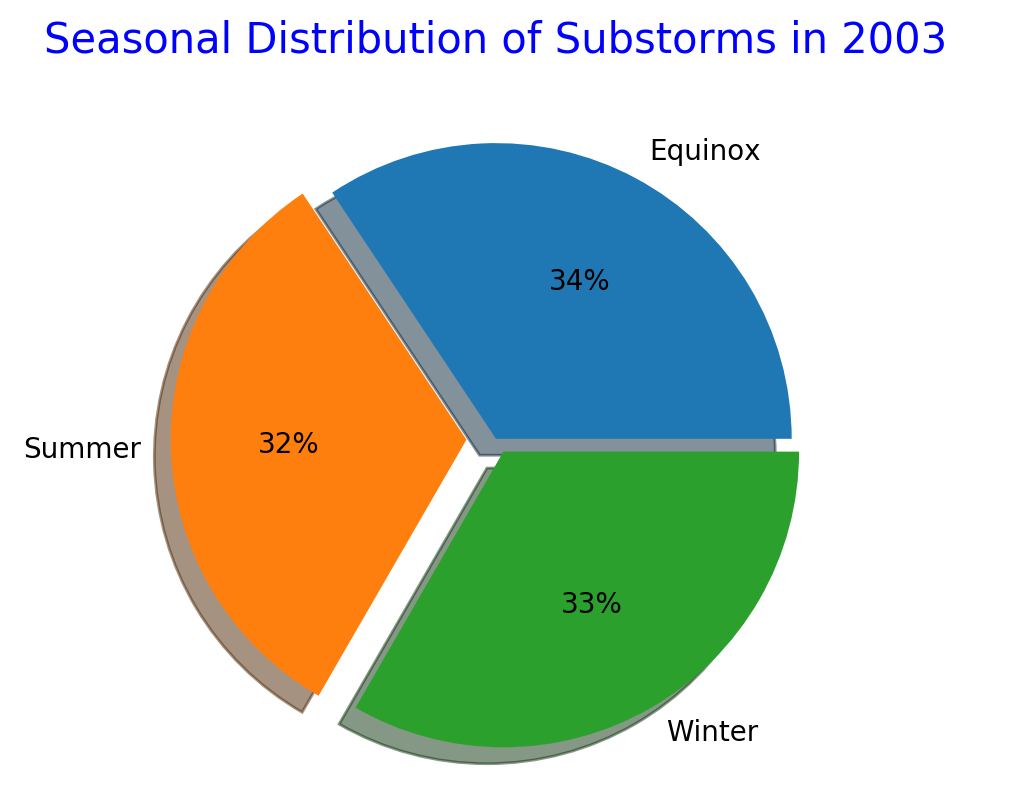
\includegraphics[width=12cm,height=6cm]{seasonal_distribution.png} % changing figure size and rotate: scale=1.2, angle=45
  \caption{Crazy Ricky and helpless Morty.} % This figure is in the same path as the code
  \label{fig:rick} % label the figure with the unique name "rick"
\end{center} % end the environment {center}
\end{figure} % end the environment {figure}


\section{Figures Environment} % Start a new section for figure
% Package 'graphicx' is needed: already loaded
\graphicspath{ {./images/} } % Added the Figure path, or you can put it directly the same path with this code
This figure \textit{\textbf{Rick and Morty }} is from my favorite American \textit{adult animation}.

The show revolves around the adventures of an eccentric and alcoholic mad scientist Rick and his grandpa Rick, 
a kind-hearted but naïve boy. Their adventures often take place across an infinite number of realities, with the 
characters travelling to other planets and dimensions through portals and Rick's flying car. Figure \ref{fig:rick} shows 
the situation in the Lab, Rick is crazy making his equipment and his grandson, Morty,is waiting helpless.

Mostly, I use the  {\tt pdflatex} command with my \textit{terminal} to compile \textit{.tex} codes. The acceptable figure 
formats are \textbf{pdf} and \textbf{png}. I also tried \textbf{jpg} format, it seems work as well. 
Figure \ref{fig:rick}! % this is the reference to the figure named "rick"
\begin{figure}[!t] % !b for bottom, t for top; ! for good position
\begin{center} % put the figure in the center 
  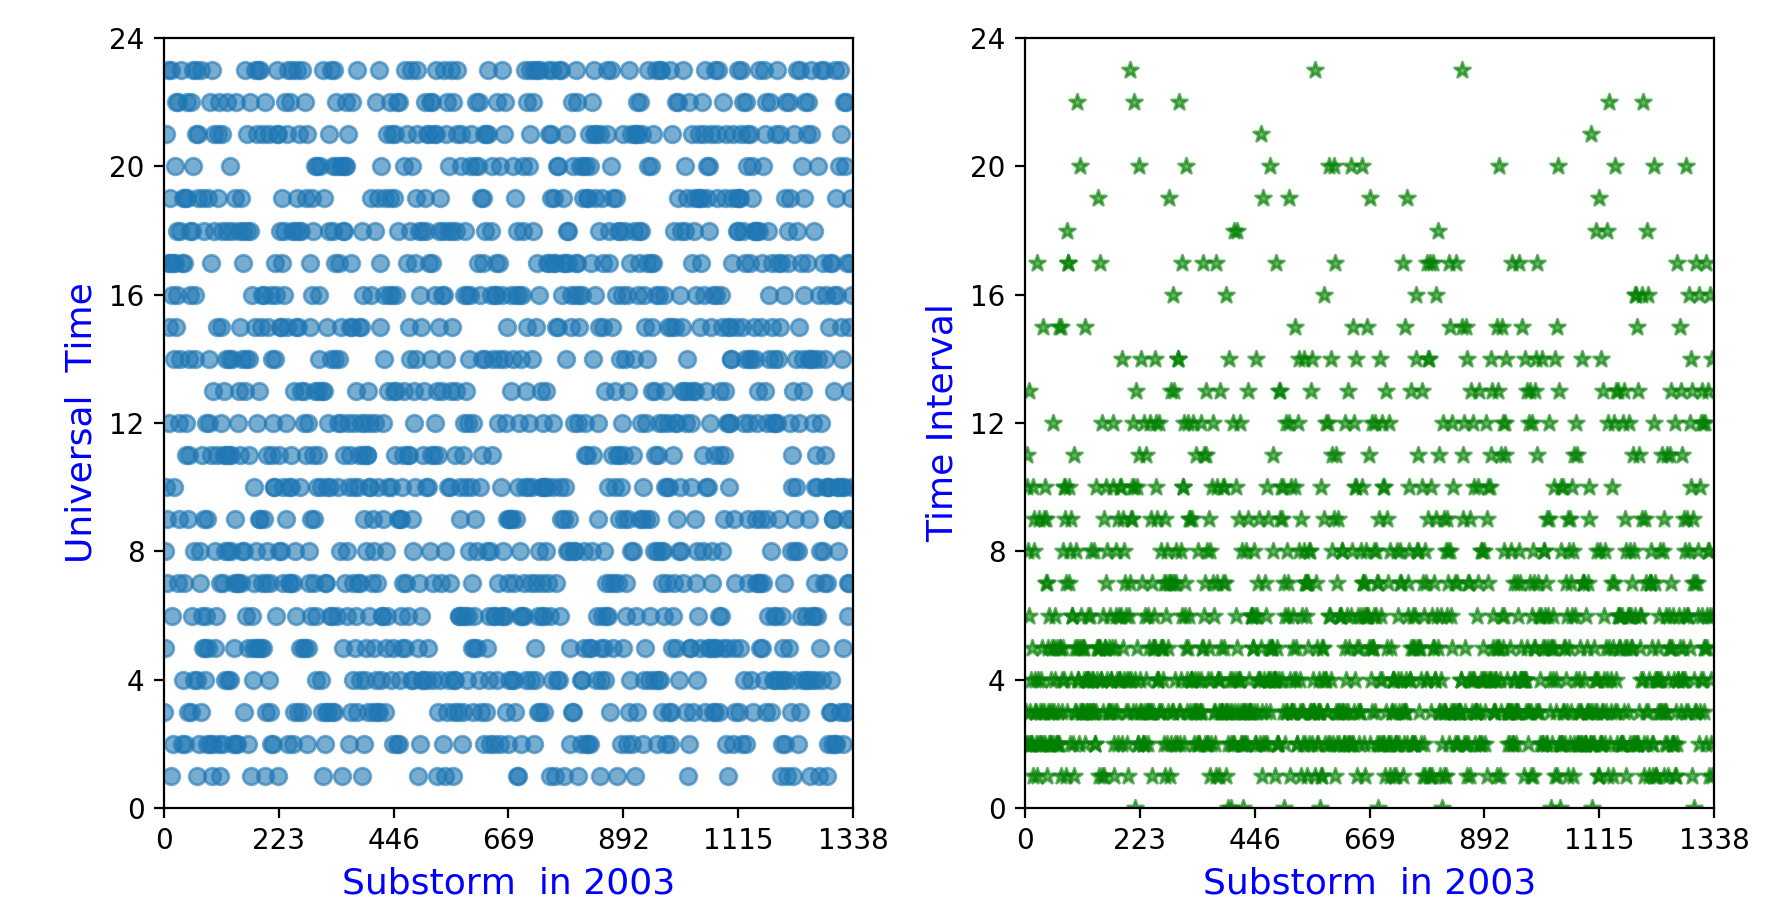
\includegraphics[width=12cm,height=6cm]{Time Interval.png} % changing figure size and rotate: scale=1.2, angle=45
  \caption{Crazy Ricky and helpless Morty.} % This figure is in the same path as the code
  \label{fig:rick} % label the figure with the unique name "rick"
\end{center} % end the environment {center}
\end{figure} % end the environment {figure}



% ============================================================================
% This Section is used for demonstrating some other useful environments in Latex
% ============================================================================
\section{Useful Environments} % Start a new section for other environments
% put contents insed \begin{envi} and \end{envi}
\begin{itemize} % This environment is used to give examples
\item[*] \textcolor{purple}{For example: itemize} % give an example
\end{itemize}  % end the environment {itemize}

\begin{abstract}  % This environment is used to set up an abstract
\begin{quote} % This environment is used to set up the cition format, similar as {quotation}
The \LaTeX  $ $ environment is a template with functions, as long as the data is entered in the prescribed format, the 
system will automatically complete the form.
\end{quote} % end the environment {quote}
\end{abstract} % end the environment {abstract}

\begin{enumerate} % This environment is used to enumerate, similar to {itemize}
\item \textcolor{green}{Another example}
\end{enumerate} % end the environment {enumerate}

\begin{center} % This environment is used to set the content centered
The typical format of commands in various environments is: 
% verbatim or verbatim* is the default tool to display code, which generates 
% an monospaced font to print exactly what you type in
\begin{verbatim} 
\begin{environment name(*)}
\begin{environment name(*)}
\end{verbatim} % end the environment {verbatim}
\end{center} % end the environment {center} 

% Using listings environment to highlight code (load the package in preamble)
\begin{lstlisting}[language=C++] 
// demo
#include <stdio.h>
int main () {
    printf("Hello world!\n");
}
\end{lstlisting}   %  end the environment {lstlisting} 

\newcommand{\myvector}[1]{${#1}_1,{#1}_2,\cdots,{#1}_n$} % define a new command "\myvector"
\myvector{a} % using my new command "\myvector"



% ===========================================================
% This Section is used to refer the figure, table, section, etc in Latex
% ===========================================================
\section{Cross-Reference!} % Start to make a new section
\label{sec:cross} % label/name this paragraph, name figures, tables, etc  in the same way
In an scientific article, we will use multiple figure \ref{fig:rick}, table \ref{tab:tab1} or cite related references 
in different part of the essay. This can be laborious! Fortunately, \LaTeX $ $ helps. If you compile this code 
successfully, you may notice that there are some interesting boxes in your .pdf file, with text in them. Please 
look at the left end of this paragraph, a box with \textsl{\textbf{sec:cross}} in side is there. Just like we people, 
we can give each figure, table quotation and whatever in your article a unique name, such as 
the section \textsl{\textbf{cross}} here. % use \ref{} to add reference to figure, table, equation, etc ....





% ===========================================================
% This Section is used for demonstrating how to create Bibliograohies in Latex
% ===========================================================
\section{Creating Bibliographies} % Start to creating Bibliograohies
\subsection{What is Bibtex ?} % subsection to introduce Bibtex
The word ,,BibTeX'' stands for a tool and a file format which are used to describe 
and process lists of references, mostly in conjunction with \LaTeX.

This is an {\it article} entry, but you can also make {\it book}, 
{\it conference}, {\it inproceedings}, and other entries.  There are many other
fields that can be filled in to make your entry more complete.  natbib provides 
three list styles: plainnat, abbrvnat, unsrtnat.

\subsection{Get Your Bibtex Files} % subsectin: how to get Bibtex files
There are many ways for getting bibtex entries: your research 
group or advisor, websites, that contains most everything.  

A bibtex file contains all of the info for any references, 
we can get this from reference management software, 
such as \textbf{Mendeley} and \textbf{EndNote}. Then 
organize the info into the following format by hand (directly):

\begin{quote} % This environment is used to set up the cition format
% The environment verbatim is used to print exactly what you type in
\begin{verbatim} 
@ARTICLE{weimer:1996,
   author = {{Weimer}, D.~R.},
    title = "{A flexible, IMF dependent model of high-latitude 
    electric potentials having "space weather" applications}",
  journal = {Geophysical Research Letters},
     year = 1996,
   volume = {23},
       doi = {10.1029/96GL02255}
}
\end{verbatim} % end the environment {verbatim}
\end{quote} % end the environment {quote}

\subsection{How to do Citations} % subsection for cases of citations
% to cite a paper, there are two common ways: \cite{} and \citep{}, just put
% the reference name (find in the Bibtex.bib file) inside the curly brackets
% for inline citation, \citet{} is usful
For high-latitude space physical environment, empirical models are very useful  
\citet{weimer:1996}. A method has been developed to derive the electric potentials 
in the high-latitude ionosphere resulting from IMF magnitude and orientation, solar 
wind velocity, and dipole tilt angle \citep[chap. 2]{weimer:1996}. In principal, this 
technique developed by {\tt weimer:1996} can be used as a forecast geomagnetic 
disturbances. Similarly, there are also several empirical models for auroral particle 
precipitation \cite[]{hardy:1989,Fuller-Rowell1987}, which are based on IMF and 
solar wind conditions as well. 

In order to fully understand the realistic process in the high-latitude ionosphere-
thermosphere system, physical modes are essentially needed. The Global Ionosphere 
Thermosphere Model (GITM) solves the complete vertical momentum equation, the 
primary characteristics of non-hydrostatic effects on the upper atmosphere are 
investigated \cite[p. 13]{Deng2008}. Meantime, the NCAR-3Dynamo model can 
be used to calculate the global ionospheric currents and magnetic disturbations 
\citep[see][chap. 5]{Maute2017}.



\subsection{Links to my Github} % start a new subsection

\begin{quote} 
% The environment verbatim is used to print exactly what you type in
\begin{verbatim}
https://github.com/Yukiooooo/PHYS-5391/tree/master/assignment-1
\end{verbatim} % end the environment {verbatim}
\end{quote} % end the environment {quote}

All the introductions are in the README.md file. 





% ===================================================
% This Section is the demonstration of  how to Use Bibtex 
% ===================================================
% for the bibliography, these two lines are Very Useful.
\clearpage % make a new page 
\addcontentsline{toc}{section}{Bibliography} % make a section in the table of contents
% Using Bibtex, we just use these two lines to add the bib!
\bibliographystyle{plainnat} % plainnat is the standard plain format
\bibliography{assignment1} % assignment1 is the name of my bibtex file

% End the document environment.  This is the last line for coding
\end{document}










